\documentclass{article}

\usepackage[utf8]{inputenc}
\usepackage[margin=3cm]{geometry}
\usepackage{graphicx}
\usepackage{minted}
\usepackage{xcolor}
\usepackage{hyperref}
\usepackage{caption}
\usepackage{amsmath}
\usepackage[backend=bibtex, style=authoryear]{biblatex}

\hypersetup{colorlinks,linkcolor=,urlcolor=,citecolor=blue}
\usemintedstyle{friendly}
\definecolor{bg}{rgb}{0.95,0.95,0.95}
\addbibresource{references.bib}

\title{Lab 07: A ``gentle'' Introduction to Artificial Neural Networks in R}
\author{Andrés Oswaldo Calderón Romero, PhD.}
\date{\today}

\begin{document}

\maketitle

\section{Core Concepts of ANN}
An Artificial Neural Network (ANN) is a set of connected input-output units where each connection has an associated weight. In the learning phase, the network adjusts these weights to predict the correct target values of input tuples.

A standard unit is a mathematical function that takes a linear weighted sum of inputs and passes it through a nonlinear activation function, such as the sigmoid function. The net input is defined as $I = \sum_{i=1}^{n} X_i w_i + b$, and the final output is $O = f(I)$ \parencite{fritsch2010neuralnet}.

\section{Environment Setup}
To begin, we utilize the ``\texttt{neuralnet}'' package \parencite{fritsch2019neuralnet}, which is designed for training multilayer feed-forward networks.

\begin{listing}[H]
    \begin{minted}[
    frame=lines,
    framesep=2mm,
    baselinestretch=1.2,
    bgcolor=bg,
    fontsize=\footnotesize
    ]{r}

# Install and load the library
if(!require(neuralnet)) install.packages("neuralnet")
library(neuralnet)

    \end{minted}
    \caption{Environment setup and library initialization. This step involves installing and loading the ``\texttt{neuralnet}'' package required for training feed-forward networks.}
\end{listing}

\section{Data Preprocessing}
Neural networks often require data to be scaled, as functions like the sigmoid (squashing) function map inputs to a range of 0 to 1.

\begin{listing}[H]
    \begin{minted}[
    frame=lines,
    framesep=2mm,
    baselinestretch=1.2,
    bgcolor=bg,
    fontsize=\footnotesize
    ]{r}

# Using the built-in iris dataset
data(iris)

# Binary classification: Is the species "setosa"?
iris$is_setosa <- ifelse(iris$Species == "setosa", 1, 0)

# Normalization to [0, 1] range
maxs <- apply(iris[, 1:4], 2, max)
mins <- apply(iris[, 1:4], 2, min)
scaled <- as.data.frame(scale(iris[, 1:4], center = mins, scale = maxs - mins))
final_data <- cbind(scaled, is_setosa = iris$is_setosa)

# Splitting into Training (70%) and Test (30%)
set.seed(42)
index <- sample(1:nrow(final_data), 0.7 * nrow(final_data))
train_set <- final_data[index, ]
test_set <- final_data[-index, ]

    \end{minted}
    \caption{Data preprocessing and partitioning. This listing covers loading the Iris dataset, performing range normalization (scaling inputs from 0 to 1), and splitting the data into training (70\%) and testing (30\%) subsets.}
\end{listing}



\section{Training the Model}
We train the network using the backpropagation algorithm, which iteratively modifies weights in a ``backward'' direction to minimize the error between predictions and actual targets.

\begin{listing}[H]
    \begin{minted}[
    frame=lines,
    framesep=2mm,
    baselinestretch=1.2,
    bgcolor=bg,
    fontsize=\footnotesize
    ]{r}

# Training a network with one hidden layer of 3 units
# This is a two-layer neural network (input layer not counted)
nn <- neuralnet(is_setosa ~ Sepal.Length + Sepal.Width + Petal.Length + Petal.Width,
                data = train_set,
                hidden = 3,
                linear.output = FALSE)

    \end{minted}
    \caption{Training the multilayer feed-forward neural network. The code demonstrates training a model with one hidden layer of three units using the backpropagation algorithm to minimize prediction error.}
\end{listing}

\section{Visualization}
The architecture of a multilayer feed-forward network consists of an input layer, one or more hidden layers, and an output layer.  Figure \ref{fig:nn} shows the architecture of the network.

\begin{listing}[H]
    \begin{minted}[
    frame=lines,
    framesep=2mm,
    baselinestretch=1.2,
    bgcolor=bg,
    fontsize=\footnotesize
    ]{r}

# Plotting the network architecture
plot(nn)

    \end{minted}
    \caption{Visualization of the network architecture. This command generates a visual representation of the input, hidden, and output layers of the trained model.}
\end{listing}

\begin{figure}
    \centering
    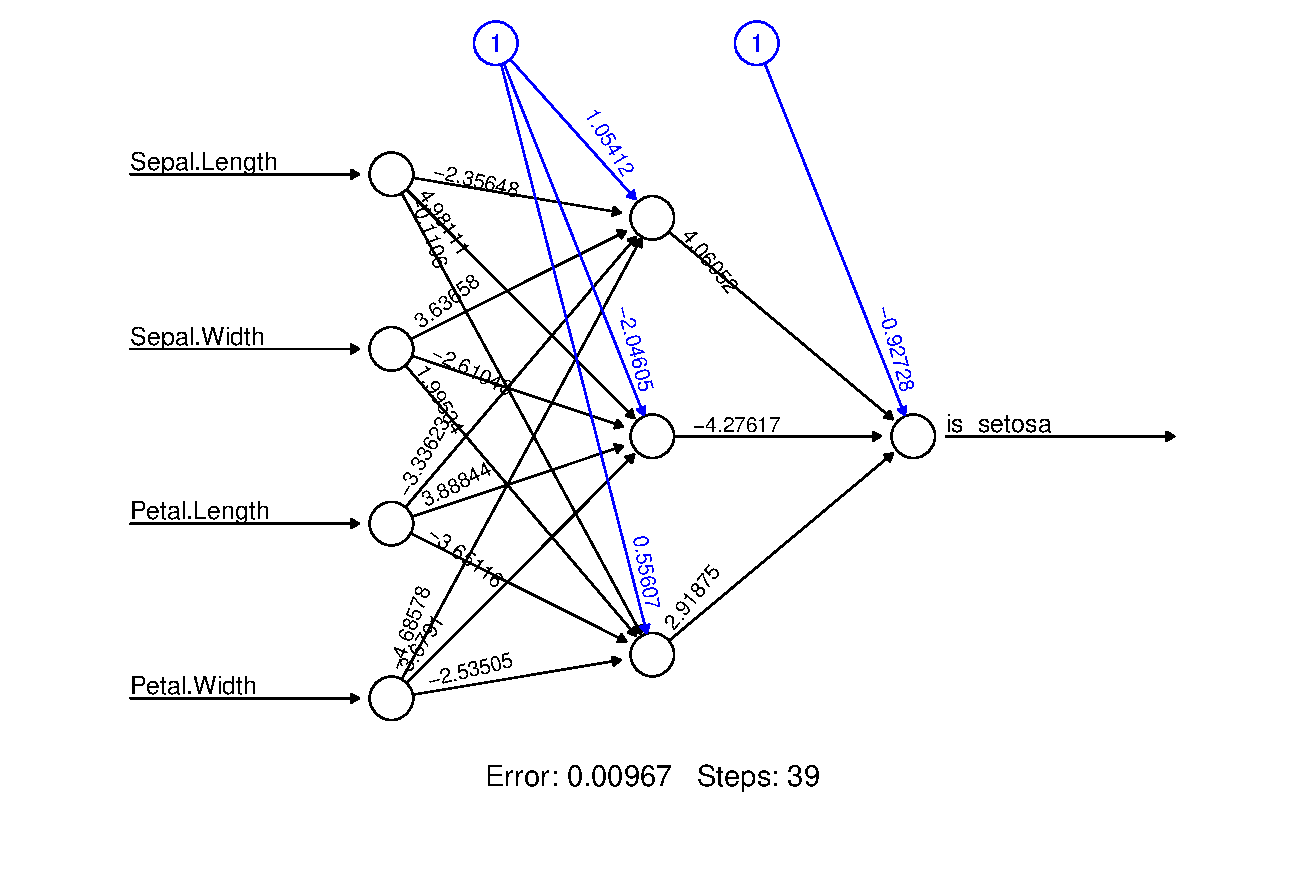
\includegraphics[width=0.8\textwidth]{figures/nn}
    \caption{This diagram illustrates a feed-forward ANN with four input nodes, a single three-unit hidden layer, and a binary output for setosa identification.  It visualizes the specific connection weights and bias values refined through training to achieve minimal prediction error.}
    \label{fig:nn}
\end{figure}

\section{Evaluation}
To classify unknown tuples, we input them into the trained network and compute the output units' values. For binary tasks, a value $\ge$ 0.5 is typically considered the positive class.

\begin{listing}[H]
    \begin{minted}[
    frame=lines,
    framesep=2mm,
    baselinestretch=1.2,
    bgcolor=bg,
    fontsize=\footnotesize
    ]{r}

# Prediction on test data
results <- compute(nn, test_set[, 1:4])
predictions <- ifelse(results$net.result > 0.5, 1, 0)

# Confusion Matrix and Accuracy
conf_matrix <- table(Actual = test_set$is_setosa, Predicted = predictions)
accuracy <- sum(diag(conf_matrix)) / sum(conf_matrix)

print(conf_matrix)
#       Predicted
# Actual  0  1
#      0 33  0
#      1  0 12

print(paste("Test Accuracy: ", round(accuracy, 4)))
#[1] "Test Accuracy:  1"

    \end{minted}
    \caption{Model evaluation and performance metrics. This section calculates predictions on test data, generates a confusion matrix, and computes the final test accuracy.}
\end{listing}

\section{Predicting New Tuples}
We can now predict the class of a new observation. Note that new data must undergo the same normalization as the training data.

\begin{listing}[H]
    \begin{minted}[
    frame=lines,
    framesep=2mm,
    baselinestretch=1.2,
    bgcolor=bg,
    fontsize=\footnotesize
    ]{r}

# New tuple: SL=5.0, SW=3.4, PL=1.5, PW=0.2
new_tuple <- data.frame(Sepal.Length=5.0, Sepal.Width=3.4, Petal.Length=1.5, Petal.Width=0.2)
new_scaled <- as.data.frame(scale(new_tuple, center = mins, scale = maxs - mins))

# Compute prediction
pred_new <- compute(nn, new_scaled)
print(paste("Probability of Setosa: ", round(pred_new$net.result, 4)))
# [1] "Probability of Setosa:  0.9897"

    \end{minted}
    \caption{Predictive inference for a new data observation. This final step scales a new data tuple and uses the trained network to compute the probability of it belonging to a specific class.}
\end{listing}

\section{Autonomous Work}

\begin{enumerate}

    \item Reproduce the Artificial Neural Network (ANN) implementation using the ``Advertisement'' dataset as detailed in Section 3 of Lab 05.

    \item Generate a confusion matrix and calculate validation metrics. Compare these results with the performance of the Decision Tree and SVM models developed in previous labs.

    \item Choose any dataset available at the UC Irvine Machine Learning Repository\footnote{\url{https://archive.ics.uci.edu/datasets/}} \parencite{Dua2019}. Replicate the procedures demonstrated in this lab to develop an interpretable ANN classifier and report all relevant evaluation metrics.

\end{enumerate}

\textit{Note: You can use the programming language of your choice.}

\printbibliography[title={References}]

\end{document}
